%\documentclass{beamer}
\documentclass[handout]{beamer}
\usetheme{boxes} 
%\usetheme{default}

%math fonts
%\renewcommand\mathfamilydefault{\rmdefault}
\usepackage{graphicx}

%page numbers
\setbeamertemplate{footline}[page number]

\setbeamercovered{invisible}
\setbeamertemplate{navigation symbols}{} 
\usepackage{mathtools}
\usepackage{graphicx}
\usepackage{amsmath}
\usepackage{epstopdf}
\usepackage{pgfplots}
\usepackage{color}
\usepackage{subfig}
\usepackage{tikzscale}
\usepackage{hyperref}
\usepackage{multimedia}
\usepackage{CJKutf8}
%\usetikzlibrary{plotmarks}

\title[Trajectory Tracking]{Optimizing Robot Striking Movement Primitives with Iterative Learning Control}
\author{Okan Ko\c c, Guilherme Maeda, Gerhard Neumann, Jan Peters}
\institute[IAS]
{
MPI for Intelligent Systems, T\"ubingen, Germany \\
Robot Learning Lab \\
\medskip
{\emph{okan.koc@tuebingen.mpg.de}}
}
\date{\today}

% custom commands
\newcommand{\boldvec}[1]{\boldsymbol{\mathrm{#1}}}
\let\vec\boldvec
\newcommand\at[2]{\left.#1\right|_{#2}} % the at differential sign
\newcommand\scalemath[2]{\scalebox{#1}{\mbox{\ensuremath{\displaystyle #2}}}} % scaling matrices

%% custom macros
\newcommand{\todo}{\textcolor{red}{TODO}} % TODO!
\newcommand{\kin}{\mathcal{T}} % used to denote inverse kinematics
\newcommand{\invKin}{\mathcal{T}^{-1}} % used to denote inverse kinematics

\newcommand{\joint}{\vec{q}} % used to denote robot state in joint space
\newcommand{\state}{\vec{y}} % denotes the generalized coordinates - joint space and velocity coordinates
\newcommand{\error}{\vec{e}} % difference between state and reference
\newcommand{\traj}{\vec{r}} % used to denote the points on the trajectory to be tracked

\newcommand{\dist}{\vec{\epsilon}} % denotes the disturbances acting on the rigid body dynamics
\newcommand{\linDist}{\vec{d}} % denotes the disturbances on the LTV model

\newcommand{\sysInput}{\vec{u}} % used to denote the system inputs
\newcommand{\linInput}{\tilde{\sysInput}} % denotes the LTV inputs
\newcommand{\trjInput}{\sysInput_{\mathrm{IDM}}} % denotes the inputs on the trajectory (calculated using IDM)
\newcommand{\ilcInput}{\sysInput_{\mathrm{ILC}}}


% % % % DMP terminology % % % %
\newcommand{\dmp}{s} % used to denote the dmp trajectory states
\newcommand{\goal}{g} % goal state
\newcommand{\force}{\mathit{f}} % forcing term of the dmps
\newcommand{\phase}{\phi} % phase of the dmp
\newcommand{\weights}{w} % weights of the dmp
\newcommand{\basis}{\Psi} % basis functions of the dmp as a matrix
\newcommand{\amp}{A} %amplitude of the rhythmic dmp
\newcommand{\basisHeight}{h} % basis fnc parameters
\newcommand{\basisCenter}{c}

% % % % ILC terminology % % % %
\newcommand{\qmatrix}{\vec{\Gamma}} % denotes the filtering qmatrix term of Bristow et al.
\newcommand{\lmatrix}{\vec{L}} % denotes the learning matrix of Bristow et al.

\newcommand{\dynamics}{\vec{f}}
\newcommand{\dynamicsNominal}{\dynamics_{\mathrm{nom}}}
\newcommand{\policy}{\vec{\pi}}
\newcommand{\ValueFunction}{J}
\newcommand{\episode}{k} % used for episode number

\newcommand{\totalTime}{T} % total time duration 
\newcommand{\numSteps}{N} % total number of time steps
\newcommand{\numepisode}{K} % total number of episodes

\newcommand{\threshold}{\epsilon}
\newcommand{\alg}{\emph{gILC}}
\newcommand{\dataset}{E}

% Set the paths where all figures are taken from:
\graphicspath{{Pictures/}}
\mathtoolsset{showonlyrefs} 
\newcommand{\includesvg}[1]{%
% \executeiffilenewer{#1.svg}{#1.pdf}%
% {inkscape -z -D --file=#1.svg %
% --export-pdf=#1.pdf --export-latex}%
 \input{#1.pdf_tex}%
} 
%\AtBeginSection{\frame{\sectionpage}}

\begin{document}
%
\begin{frame}
\titlepage
\end{frame}
%
\begin{frame}
\frametitle{Table of Contents}
\tableofcontents
\end{frame}
%
\section{Motivation: Imitation Learning}
%
\begin{frame}{Setup}
\begin{itemize}
\item We give the robot reference trajectories that facilitate good striking motions. We can teach the robot such trajectories via kinesthetic teach-in.
\end{itemize}
\begin{figure}[b!]
\centering
\movie[externalviewer]{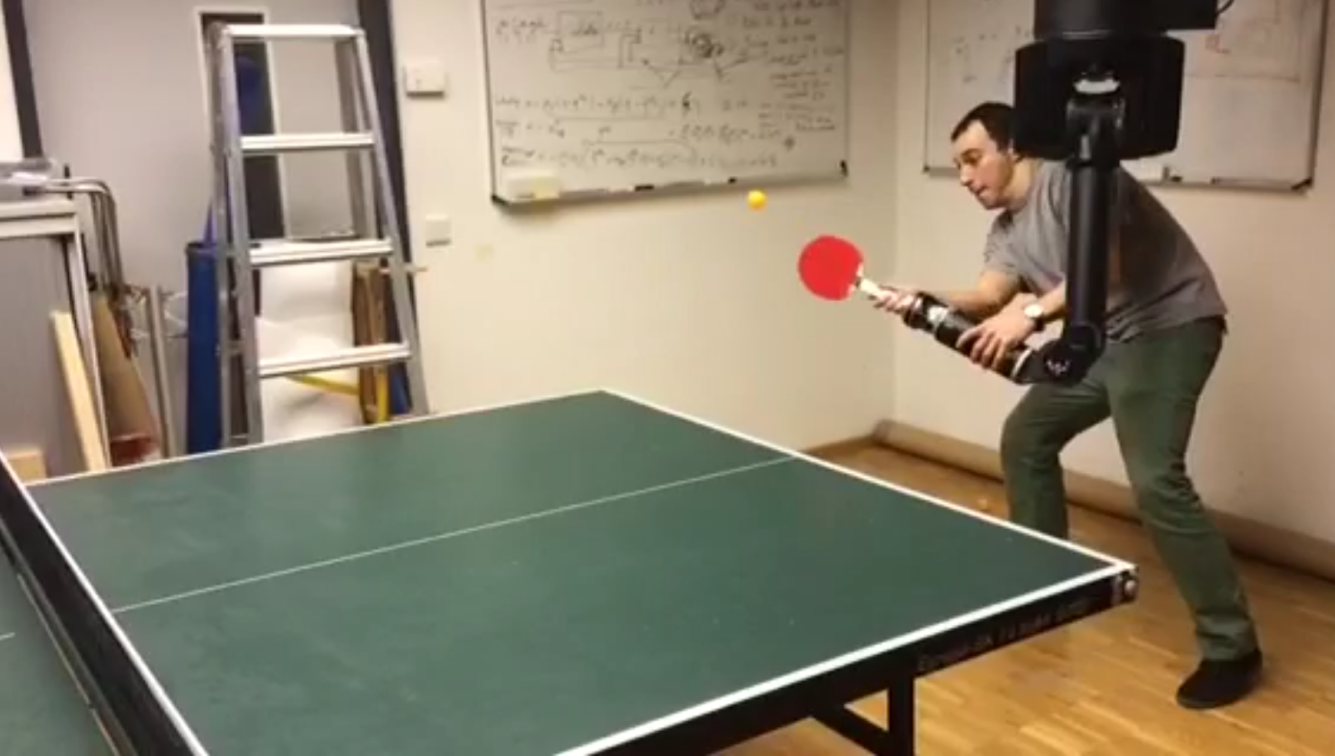
\includegraphics[scale=0.3]{demonstrations.png}}{okanTeachINSlowMotion.MOV}
%\caption{In slow motion we can see better how the joints are being moved.}
\end{figure}
\end{frame}
%
\section{Movement Primitives}
%
\begin{frame}{Movement Primitives}
\begin{itemize}
\item Dynamic Movement Primitives (DMP) are a dynamical systems based approach to parametrize trajectories
\begin{equation}
\begin{aligned}
\dot{\dmp} &= \vec{A}_s \dmp + \basis(\phase) \weights, \\
\dot{\phase} &= \tau.
\label{dmp1}
\end{aligned}
\end{equation}
\item Rhythmic DMPs can represent striking movements taught with imitation learning by regressing $\weights$ on sample trajectories.
\item As phase $\phase$ progresses, the state $\dmp$ is attracted to a limit cycle enforced by $\force(\phase) = \basis(\phase)\weights$
\end{itemize}
\begin{figure}
\center
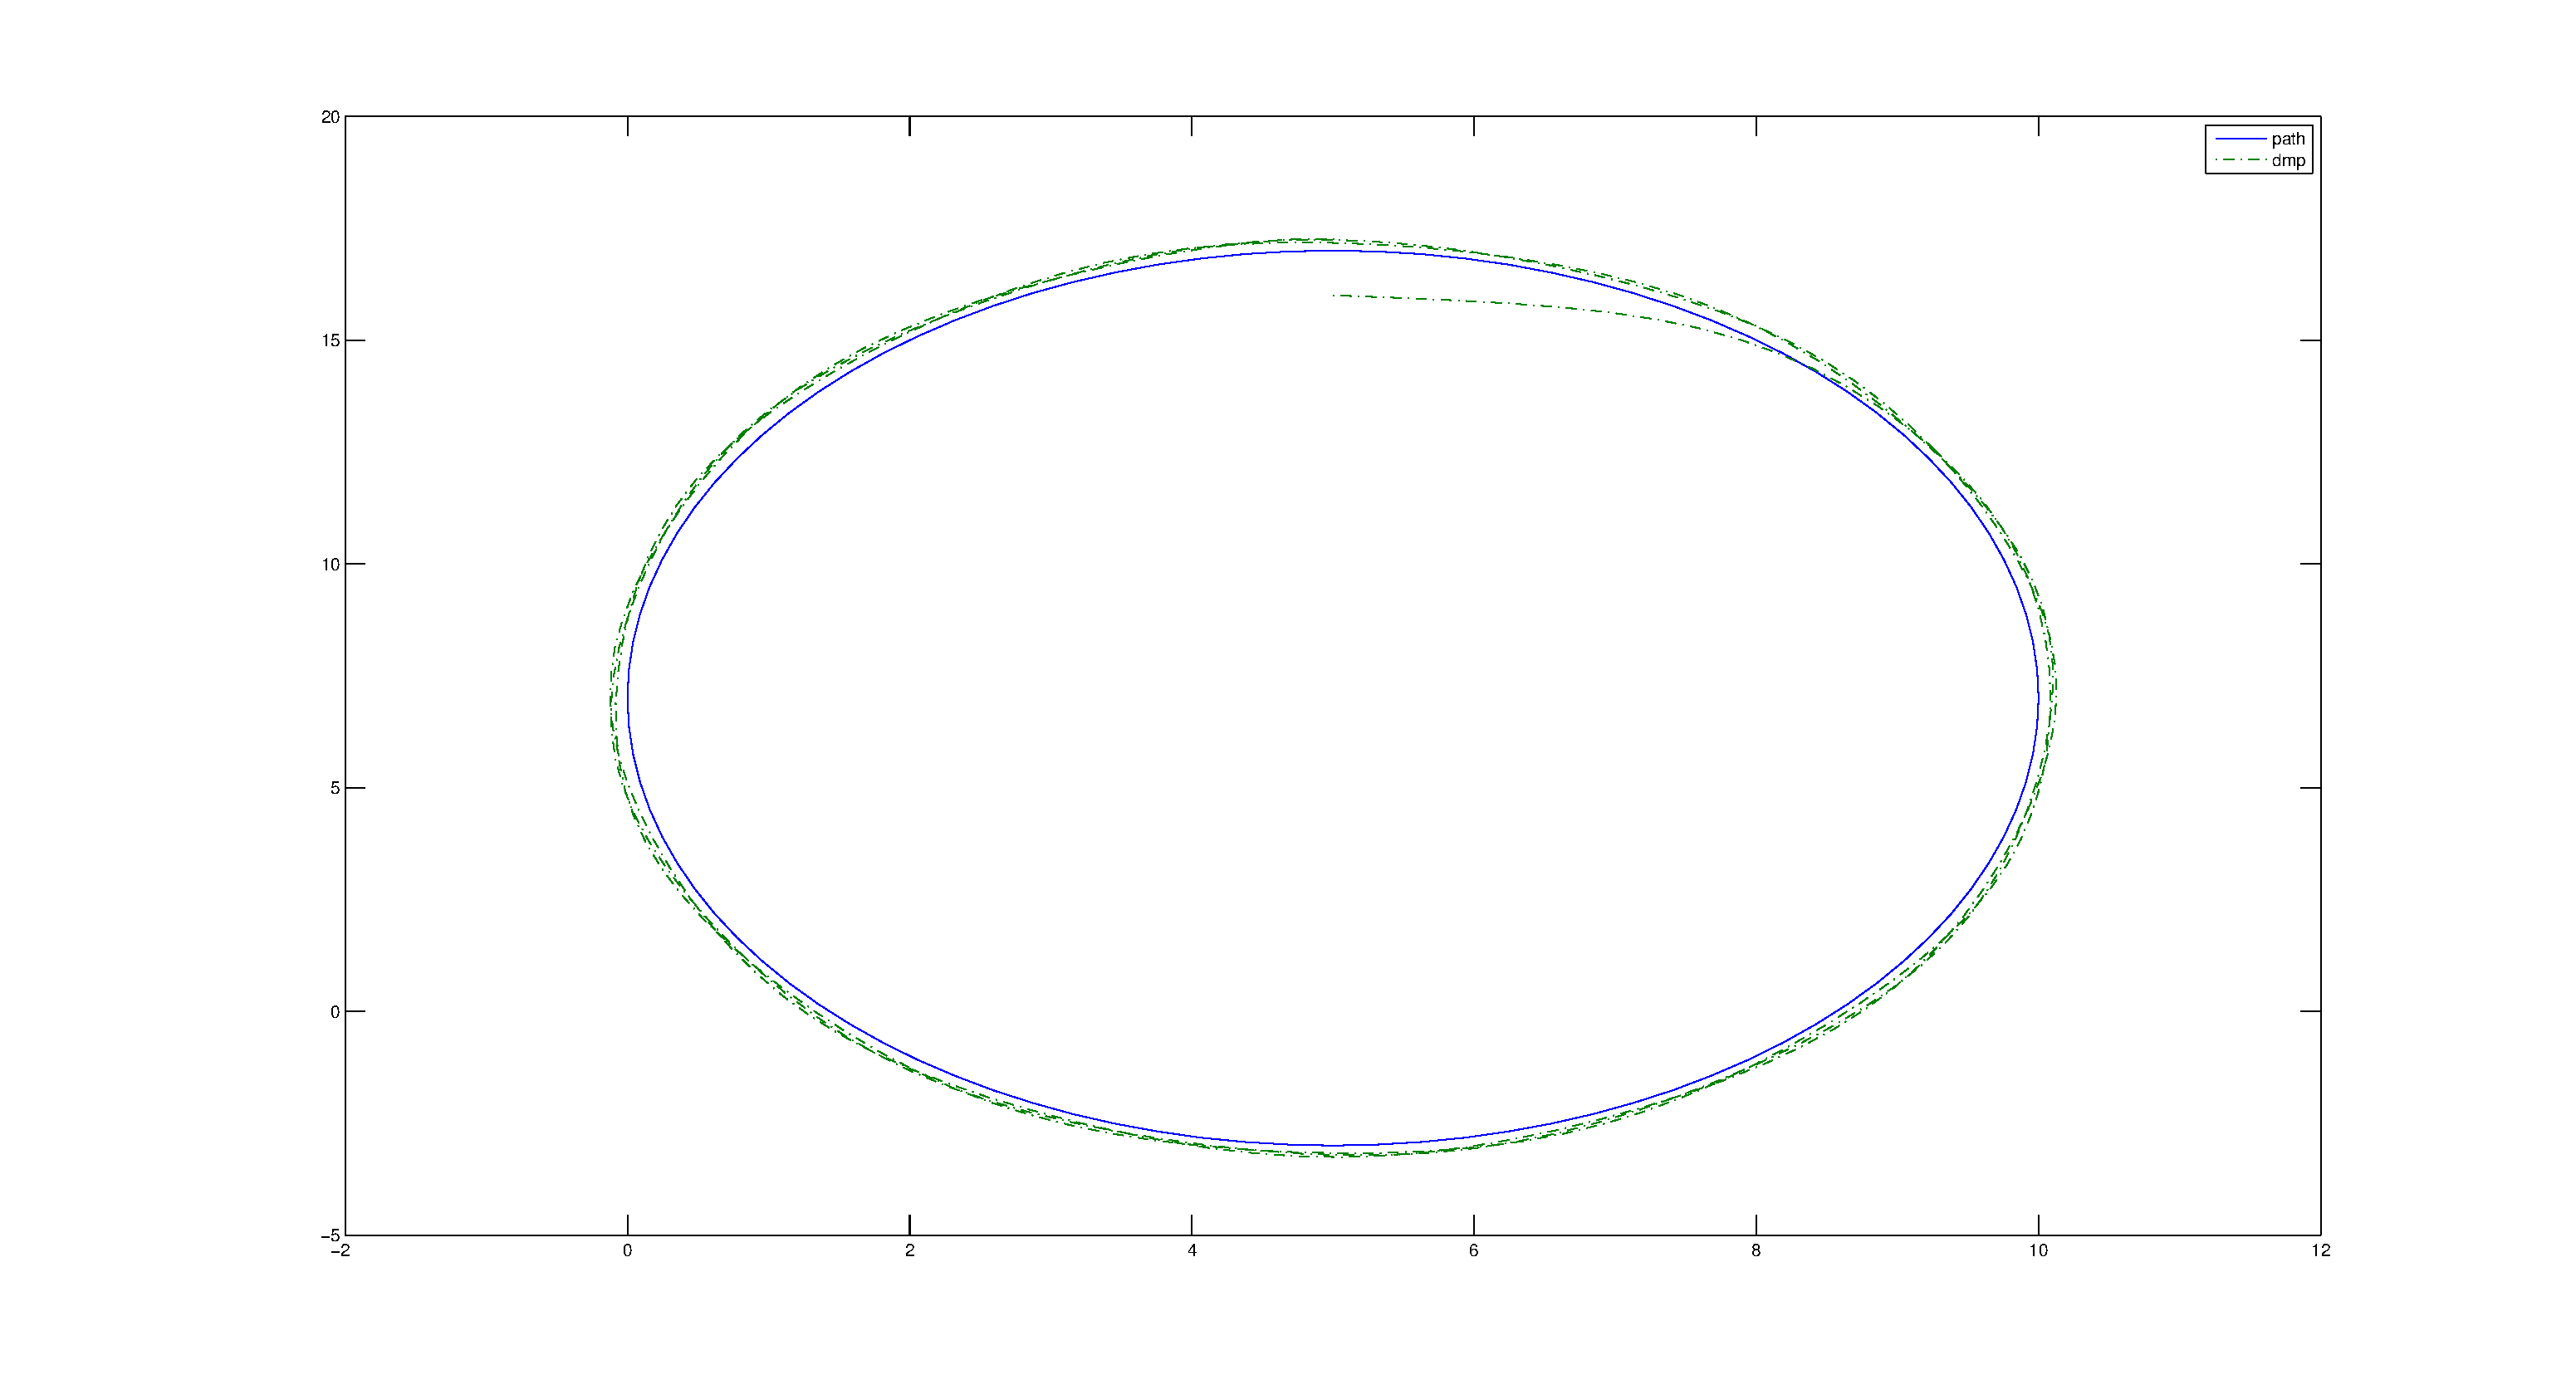
\includegraphics[scale=0.15]{rdmp0.eps}			
%\caption{DMP following a certain path.}
\end{figure}
\end{frame}
%
\begin{frame}{Research Question}

\begin{itemize}
\item Approximation and control errors in table tennis make the application of DMPs less useful in practice.
\item How can we learn to hit optimally, while efficiently exploiting an inaccurate dynamics model in a stable
way?
\end{itemize}
\begin{figure}
\center
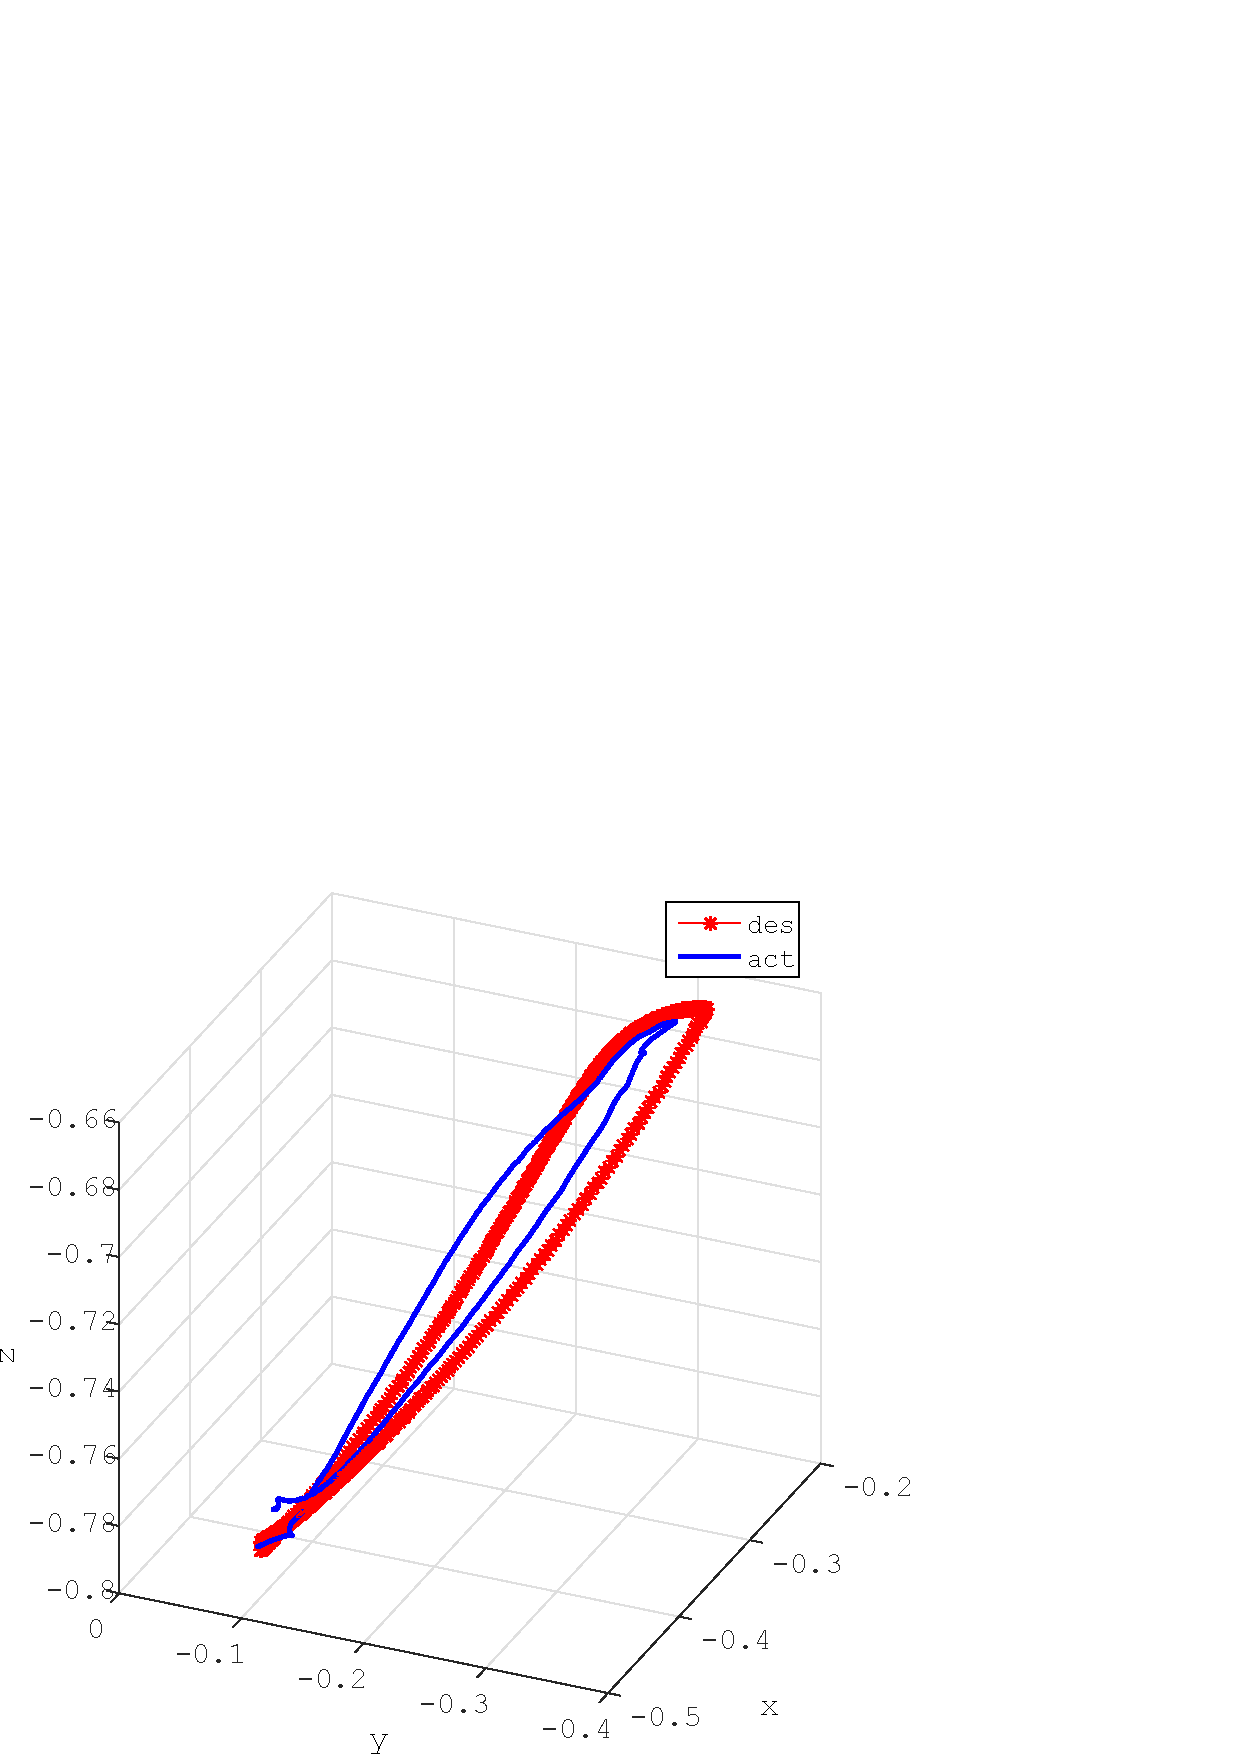
\includegraphics[scale=0.20]{rdmp.pdf}			
%\caption{DMP following a certain path.}
\end{figure}
\end{frame}
%
\section{Iterative Learning Control}
%
\begin{frame}{Iterative Learning Control (ILC)}
\begin{itemize}
\item Task: track a reference trajectory $\traj(t), \ 0 \leq t \leq T \ $ under unknown repeating disturbances or model mismatch.
\item Feedforward control inputs $\sysInput(t)$ are adjusted after each iteration. The goal is drive the deviations from the trajectory to zero. 
\end{itemize}
\begin{figure}
\center
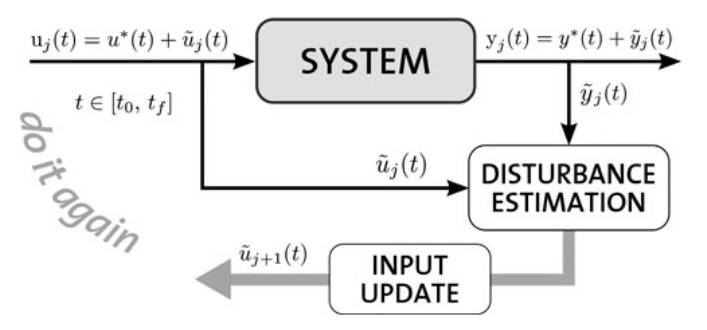
\includegraphics[scale=0.25]{ilc_framework}			
\caption{ILC Framework}
\end{figure}
\end{frame}
%
\begin{frame}{Iterative Learning Control (ILC)}
\begin{itemize}
\item A very simple update rule is to use the error $\error_k = \state_k - \traj$ and its derivatives. For example:
\begin{equation*}
\begin{aligned}
\sysInput_{k+1} = \sysInput_{k} + K_{p}\error_k + K_{d}\dot{\error}_k
\end{aligned}
\end{equation*}
\item It can easily lead to unstability! Model based update laws can be much more effective in practice!
\end{itemize}
\begin{figure}
\center
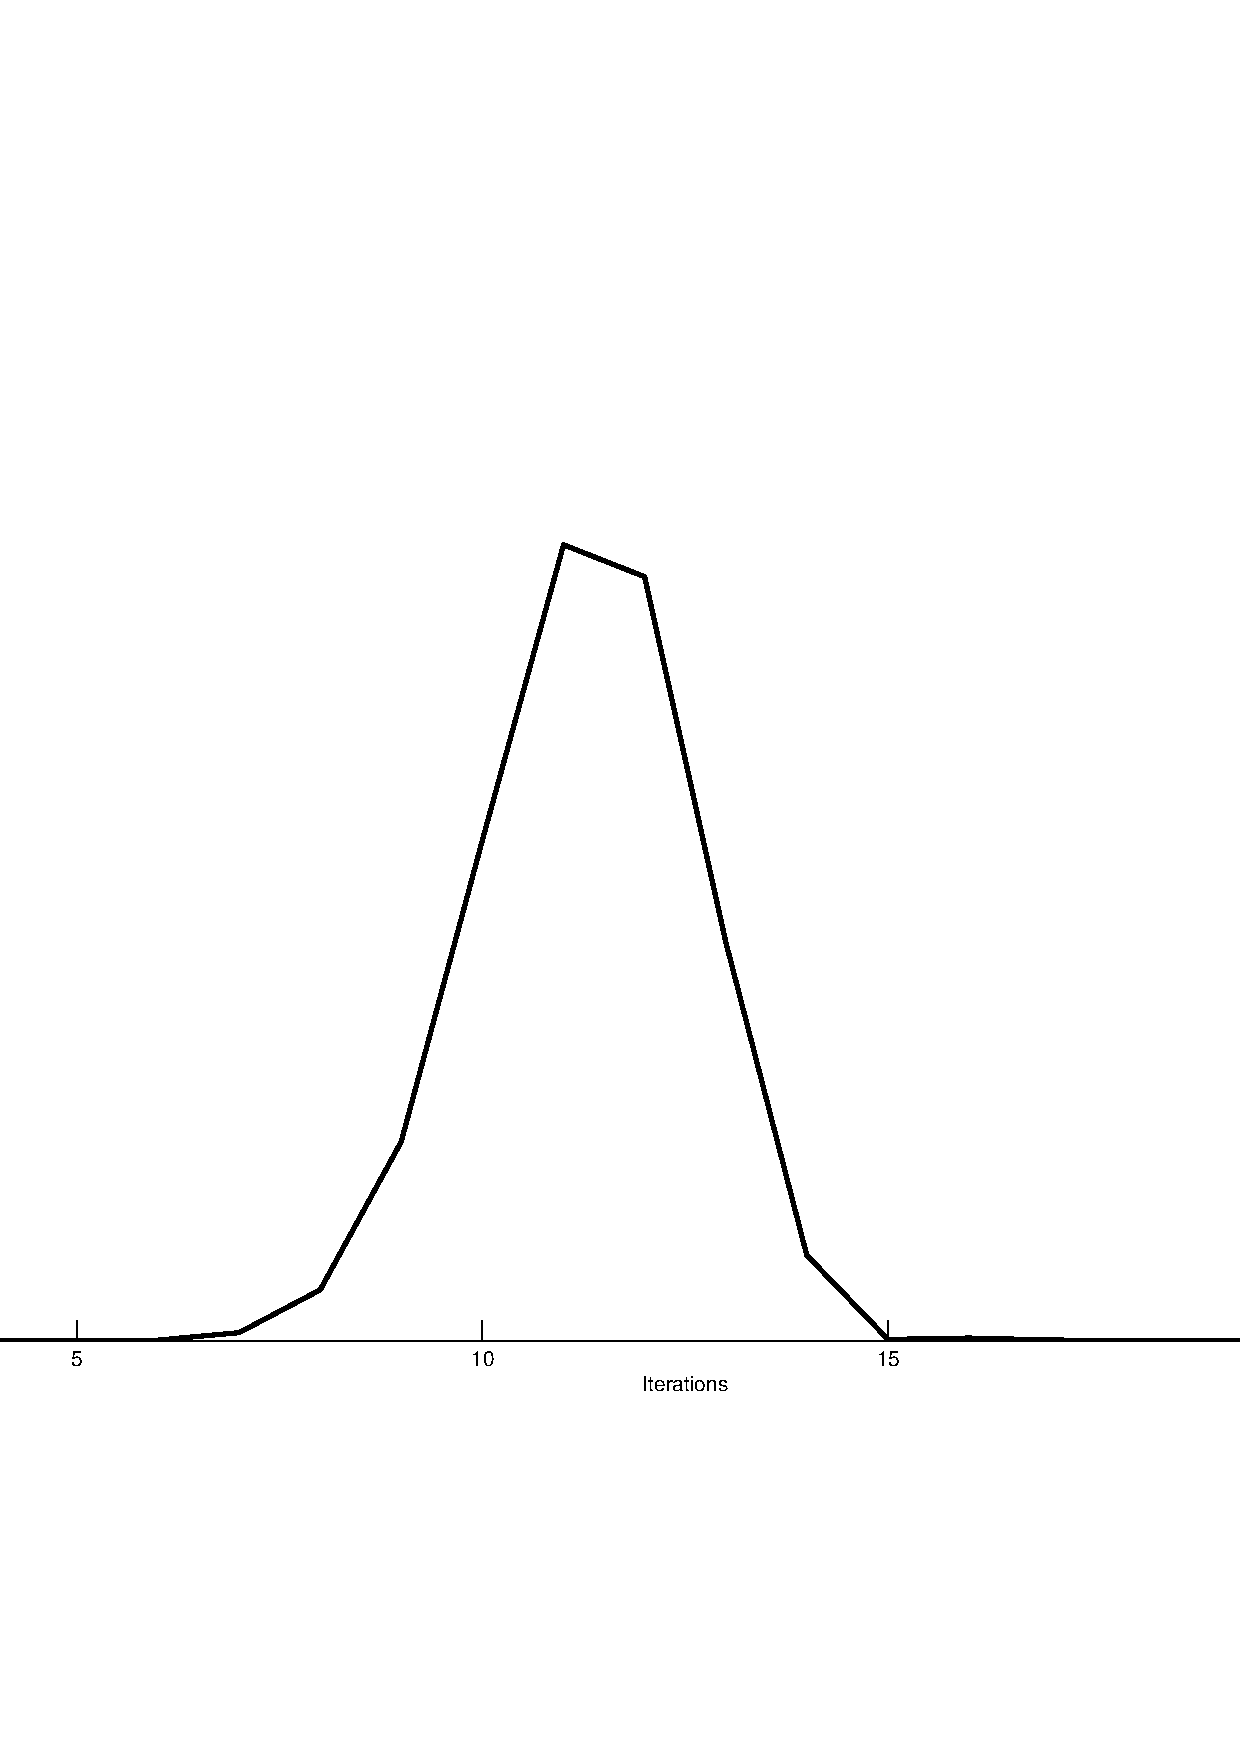
\includegraphics[scale=0.15]{ilcBlowup.pdf}			
%\caption{Naive ILC Implementation}
\end{figure}
\end{frame}
%
%
\begin{frame}{What do we need to apply models in ILC?}
\begin{itemize}
\item An \emph{approximate} inverse dynamics model:
\end{itemize}
\begin{equation*}
\begin{aligned}
M(\joint)\ddot{\joint} + C(\joint,\dot{\joint})\dot{\joint} + G(\joint) = \tau \\
\sysInput_{IDM} = \vec{f}_{inv}(\joint,\dot{\joint},\ddot{\joint})
\end{aligned}
\end{equation*}
\begin{itemize}
\item A robustly stabilizing feedback on the robot
\begin{equation*}
\begin{aligned}
\sysInput_{FB} &= -\vec{K}_{LQR}(\joint - \joint_{des})
\end{aligned}
\end{equation*}
\item Linearize the dynamics around the reference trajectory $\traj(t) = [\joint_{des}, \dot{\joint}_{des}]$ and invert it to obtain $\lmatrix$. Now we can apply ILC to the control inputs
\end{itemize}
\begin{equation*}
\begin{aligned}
\sysInput_{k+1} &= \sysInput_{k} - \lmatrix\error_{k}
\end{aligned}
\end{equation*}
\end{frame}
%
\begin{frame}{Goal-based ILC 1/2: Simulation Results}
\begin{itemize}
\item Such plant-inversion based ILC approaches may not be stable for long trajectories with different initial conditions and high mismatches!
\item Solution:
\begin{enumerate}
\item We only need to consider the hitting point(s) not the whole trajectory for successful hitting.
\item For different initial conditions, we use the DMP to converge to the desired limit cycle.
\item For additional stability we add \emph{current-iteration} ILC based on feedback: $\sysInput_{k+1} = \sysInput_{k} - K_{LQR}\error_{k}$.
\end{enumerate}
\begin{figure}
\center
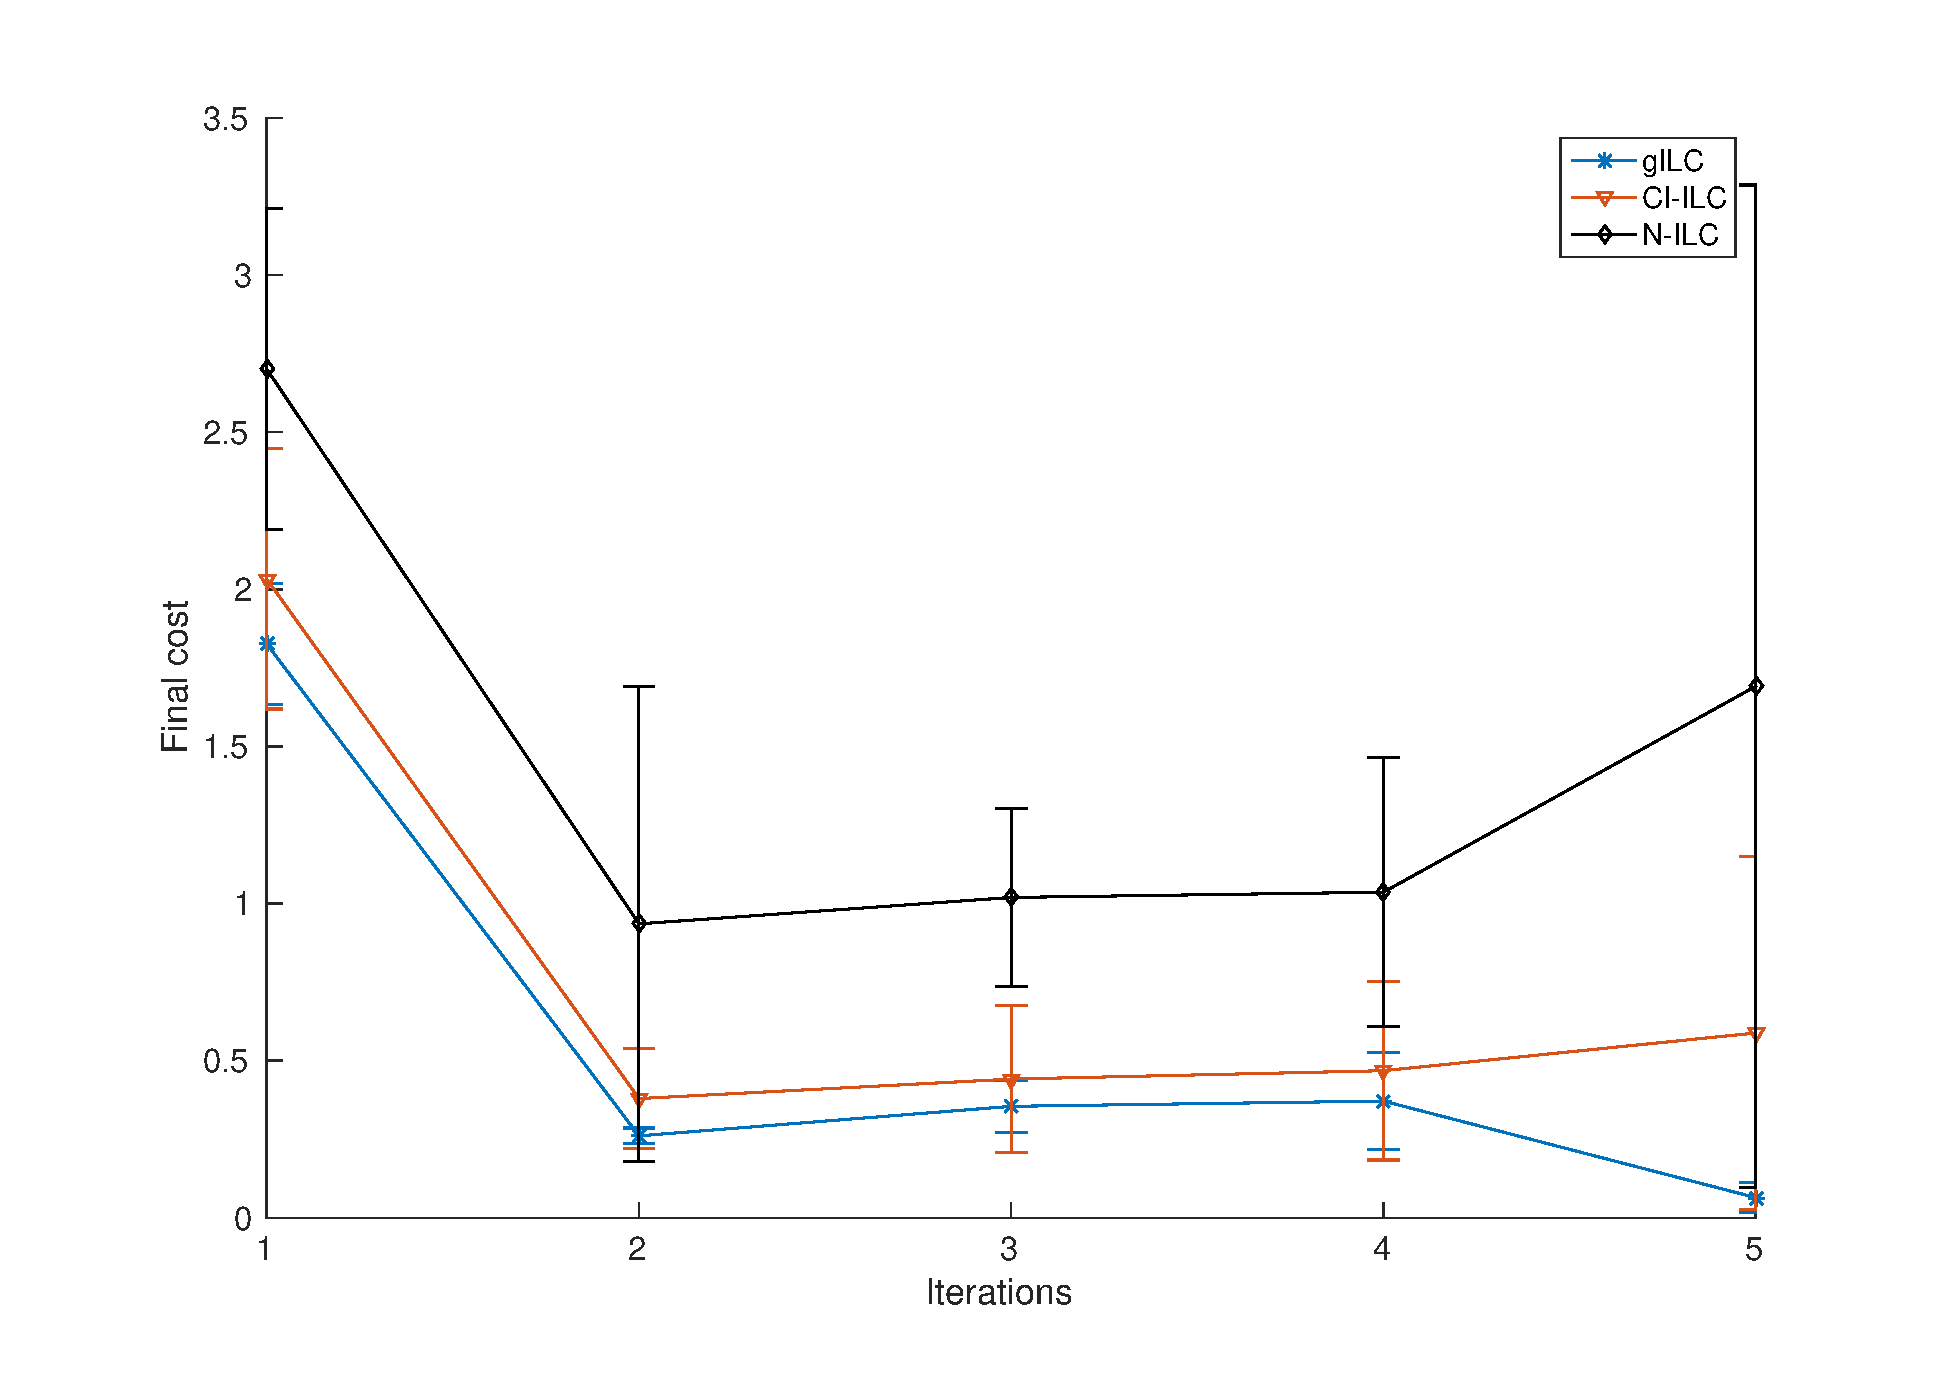
\includegraphics[scale=0.20]{ilcForWAM.eps}			
%\caption{Simulation results for goal-based ILC with Barrett WAM}
\end{figure}
\end{itemize}
\end{frame}
%
\begin{frame}{Goal-based ILC 2/2: Real robot experiment}
\begin{figure}[ht]
\centering
\subfloat{%
\includegraphics[width=0.6\linewidth]{actualResult.eps}}
\subfloat{%
\movie[externalviewer]{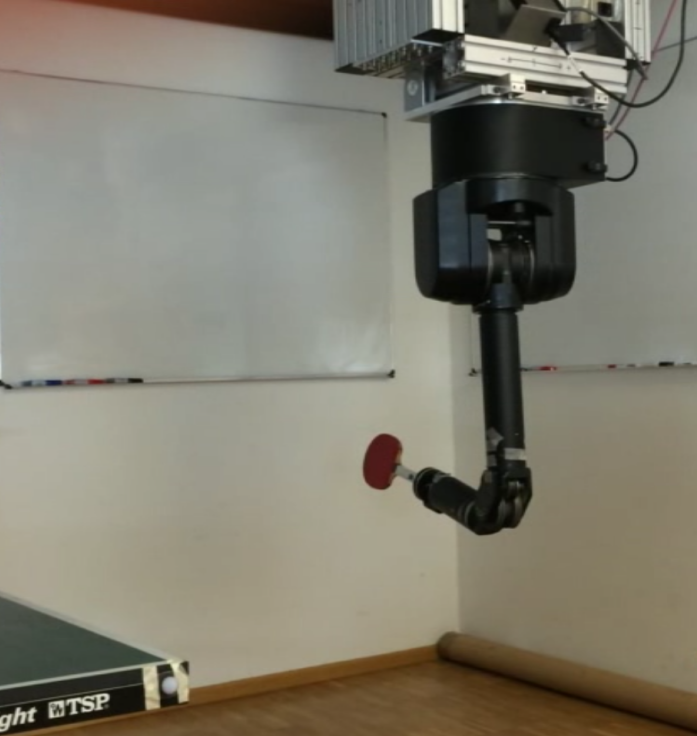
\includegraphics[scale=0.3]{ilcBarrettWAM.png}}{ilcBarrettWAM.mp4}}
%\caption{DMPs are nice!} 
\label{Robot experiment} 
\end{figure}
\end{frame}
%
\begin{frame}{Future Work}
\begin{itemize}
\item For table tennis one needs to consider parameterized trajectories with different goal states!
\item DMPs are useful for that!
\end{itemize}
\begin{figure}[b!]
\centering
\movie[externalviewer]{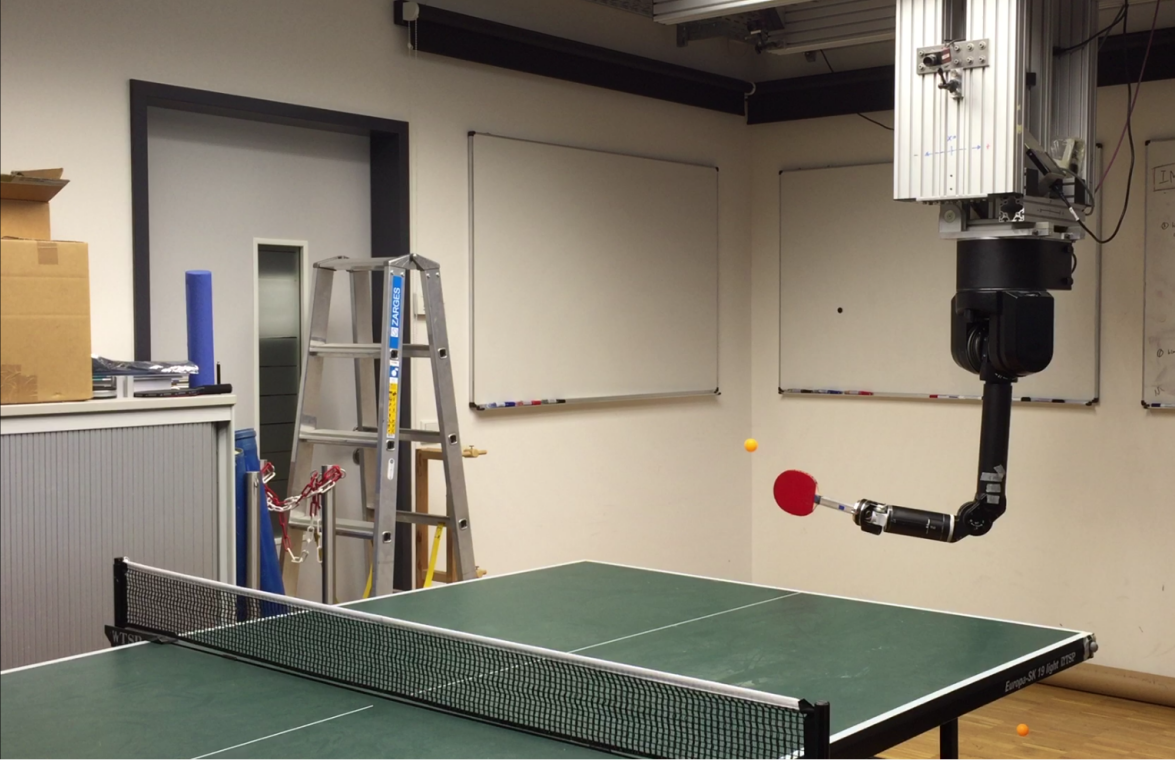
\includegraphics[scale=0.3]{tableTennis.png}}{tableTennis.MOV}
\label{Robot table tennis}
\caption{Robotic table tennis}
\end{figure}
\end{frame}
%
\begin{frame}{The End}
That's it! Gamsahabnida!
\begin{CJK}{UTF8}{mj}
감사합니다
\end{CJK}
\end{frame}
%
\section*{Appendix}
%
% End of slides
%
\begin{frame}{Discrete Movement Primitives}
\begin{itemize}
\item In discrete Dynamic Movement Primitives (dDMP), as phase $\phase$ decays, the state $\dmp$ is attracted to the goal state $\goal$ and follows a particular path along the way.
\end{itemize}
\begin{equation}
\begin{aligned}
\dot{\dmp} &= \vec{A}_s \dmp + \basis(\phase) \weights, \\
\dot{\phase} &= -\tau\alpha\phase.
\label{dmp1}
\end{aligned}
\end{equation}
\begin{figure}[ht]
\centering
\subfloat[Starting from a different initial position]{%
\includegraphics[width=0.4\linewidth]{dmp2.pdf}}
\subfloat[Stretching a DMP to a different goal position]{%
\includegraphics[width=0.4\linewidth]{dmp3.pdf}}
%\caption{DMPs are nice!} 
\label{niceDMPs} 
\end{figure}
\end{frame}
%
\begin{frame}{Rhythmic Movement Primitives}
\begin{itemize}
\item In rhythmic Dynamic Movement Primitives (rDMP), as phase $\phase$ progresses, the state $\dmp$ is attracted to a limit cycle enforced by $\force(\phase) = \basis(\phase)\weights$
\end{itemize}
\begin{equation}
\begin{aligned}
\dot{\dmp} &= \vec{A}_s \dmp + \basis(\phase) \weights, \\
\dot{\phase} &= \tau.
\label{dmp1}
\end{aligned}
\end{equation}
\begin{figure}
\center
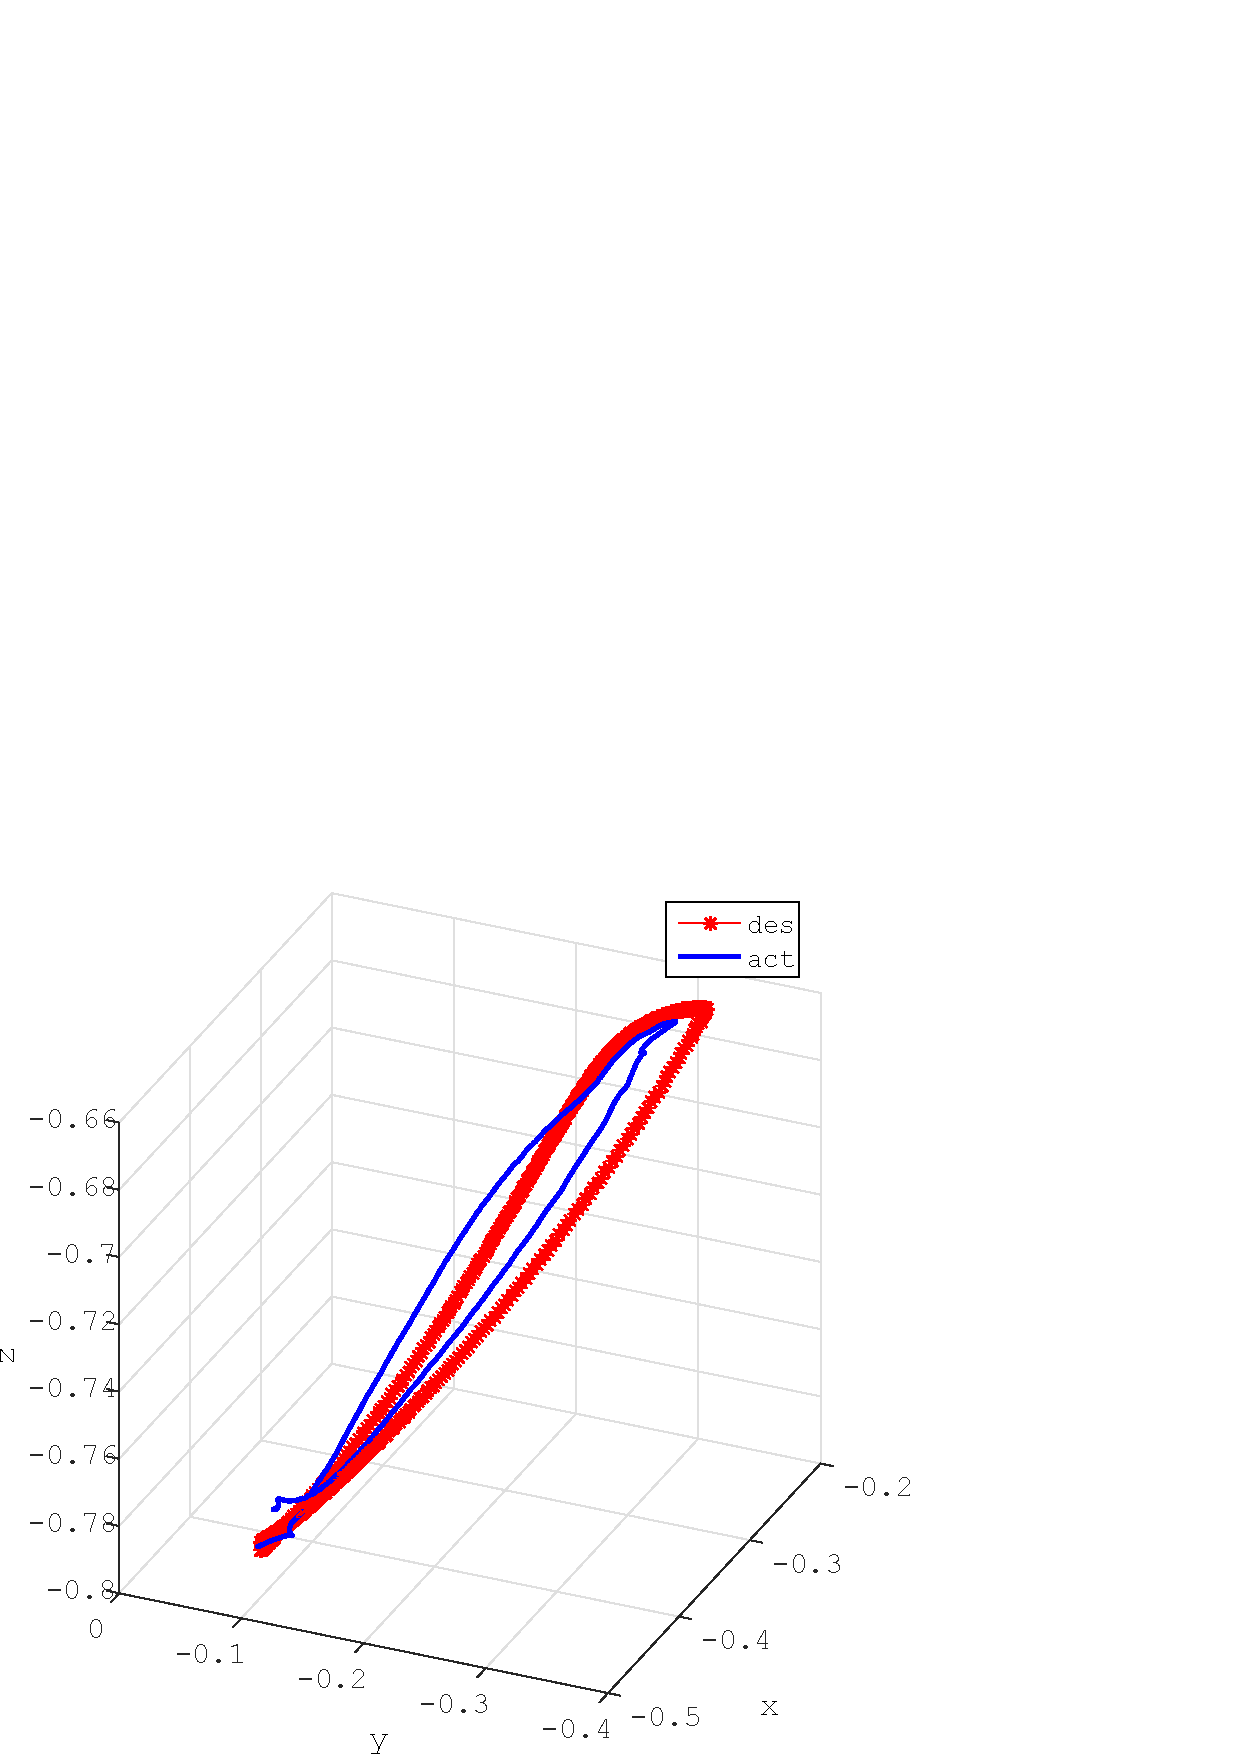
\includegraphics[scale=0.20]{rdmp.pdf}			
%\caption{DMP following a certain path.}
\end{figure}
\end{frame}
%
\begin{frame}{Linearizing around reference}
\begin{itemize}
\item Linearize the dynamics around the reference trajectory to obtain the time varying matrices $\vec{A}(t), \vec{B}(t)$
\end{itemize}
\begin{equation*}
\begin{aligned}
\dot{\error} &= \vec{A}(t)\error(t) + \vec{B}(t)\sysInput(t) + \linDist(t)\\
\end{aligned}
\end{equation*} 
\begin{itemize}
\item The time variant matrices are linearizations of $\dynamics$ 
\end{itemize}
\begin{equation*}
\begin{aligned}
\vec{A}(t) & = \at{\frac{\partial{\mathbf{f}}}{\partial{\state}}}{(\traj(t),\sysInput_{IDM}(t))} \\
\vec{B}(t) & = \at{\frac{\partial{\mathbf{f}}}{\partial{\sysInput}}}{(\traj(t),\sysInput_{IDM}(t))} \\
\end{aligned}
\end{equation*}
\begin{itemize}
\item We discretize these matrices to construct the learning matrix $L$! 
\end{itemize}
\end{frame}

\begin{frame}{Discretizing a linearized model}
\begin{itemize}
\item For j $\in \{ 1, 2, \ldots, N \}$, 
\end{itemize}
\begin{equation*}
\begin{aligned}
\error_{j+1} &= \vec{A}_j\error_j + \vec{B}_j\sysInput_j \\
\end{aligned}
\end{equation*}
\begin{itemize}
\item The discretized matrices can be found using: 
\linebreak
\end{itemize}
\begin{equation*}
\begin{aligned}
\exp^{h
\left[
\scalemath{0.5}{
\begin{array}{c|c}
A(jh) & B(jh) \\ \hline
0 & 0
\end{array}}\right]}
&= 
\left[
\begin{array}{c|c}
\vec{A}_j & \vec{B}_j \\ \hline
0 & I
\end{array}\right]
\end{aligned}
\end{equation*}
\end{frame}
%
%
\begin{frame}{Model-based ILC 1/2: Plant-inversion}
More specifically
\begin{itemize}
\item For the linearized system $\error_{j+1} = \boldvec{A}_j\error_j + \boldvec{B}_j\sysInput_j$,
\item Construct $\vec{F}$ using the model matrices $\vec{A}_j$, $\vec{B}_j$
\item $\vec{F}$ is the plant dynamics in the \emph{lifted} domain: $\state_k = \vec{F}\sysInput_k + \linDist_k$
\item With plant inversion $\lmatrix$ is the pseudoinverse of $\vec{F}$: $\sysInput_{k+1} = \sysInput_{k} - \vec{F}^{\dagger}\error_{k}$
\end{itemize}
\end{frame}
%
\begin{frame}{Model-based ILC 2/2: Norm-optimal ILC}
\begin{itemize}
\item Using the cost functional as our optimality criterion
\begin{equation}
\begin{aligned}
\ValueFunction &= \sum_{j=1}^{N} \error_j^{\mathrm{T}}\vec{Q}\error_j + \linInput_j^{\mathrm{T}}\vec{R}\linInput_j = \error_k^{\mathrm{T}}\vec{Q}_L\error_k + \sysInput_k^{\mathrm{T}}\vec{R}_{L}\sysInput_k
\end{aligned}
\end{equation}
\item With Newton's method we get
\end{itemize}
\begin{equation*}
\begin{aligned}
\sysInput_{k+1} &= \qmatrix(\sysInput_{k} - \lmatrix\error_{k}), \\
\qmatrix &= (\vec{F}^{\mathrm{T}}\vec{Q}_L\vec{F} + \vec{R}_L)^{-1}\vec{F}^{\mathrm{T}}\vec{Q}_L\vec{F}, \\
\lmatrix &= (\vec{F}^{\mathrm{T}}\vec{Q}_L\vec{F})^{-1}\vec{F}^{\mathrm{T}}\vec{Q}_L \\
\vec{F}_{(i,j)} &= \left \{
\begin{array}{cc}
\vec{A}_{i-1}\ldots \vec{A}_j\vec{B}_{j-1}, & j < i \\ 
\vec{B}_{j-1}, & j = i \\
\vec{0}, & j > i 
\end{array} \right.
\end{aligned}
\end{equation*}
\end{frame}
%
\begin{frame}{An intuitive way to understand ILC}
\begin{itemize}
\item Least squares regression on the disturbances estimated using the previous trial
\end{itemize}
\begin{equation}
\begin{aligned}
\vec{F}\sysInput_{k+1} &\approx -\linDist_{k}, \\
\sysInput_{k+1} &= \vec{F}^{\dagger}(\vec{F} \sysInput_k - \error_k).
\end{aligned}
\end{equation}
\end{frame}
%
\begin{frame}{Toy Example: Putting}
\begin{itemize}
\item Task: follow a pre-assigned trajectory (blue dashed curve) to give the golf ball the right velocity at impact.
\end{itemize}
\begin{figure}[ht]
\centering
\subfloat[Initial attempt]{%
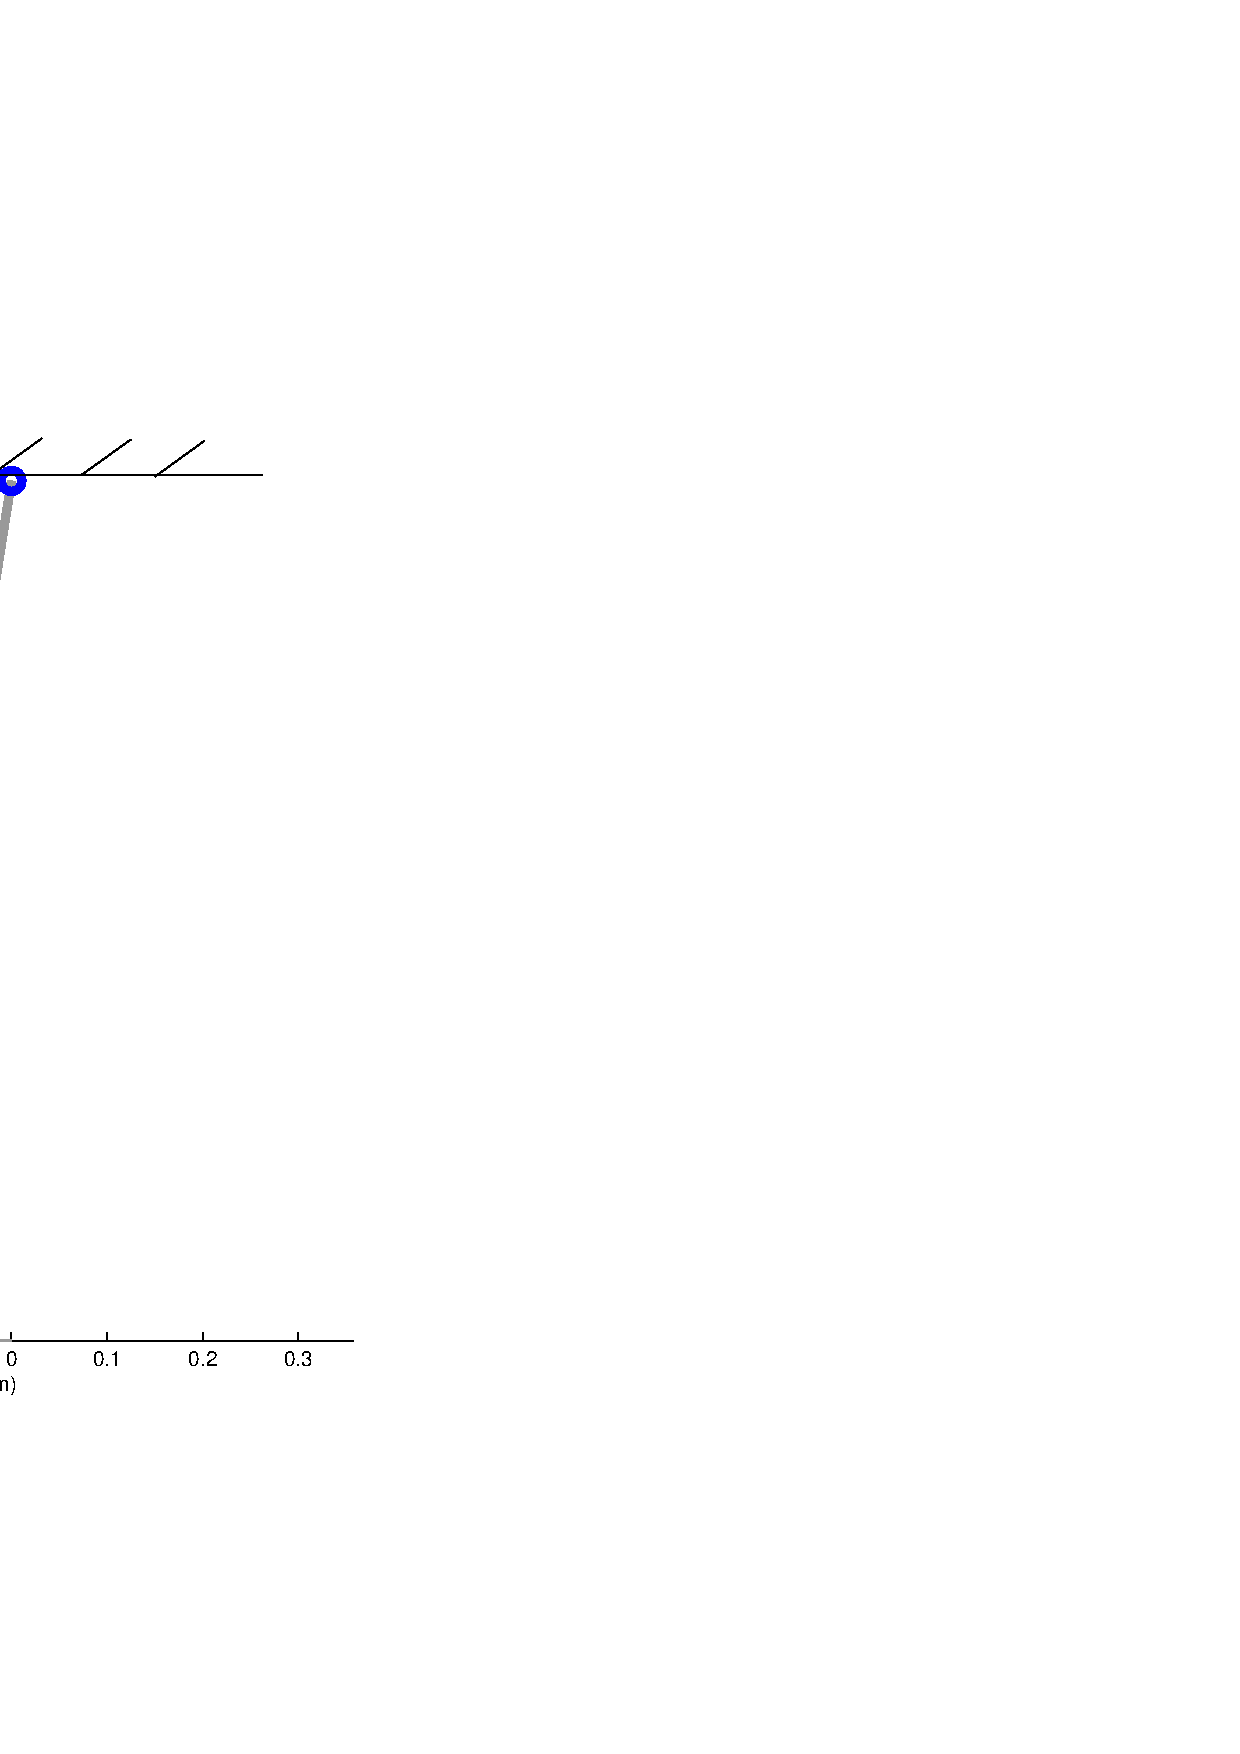
\includegraphics[width=0.3\linewidth]{putting0.pdf}
\label{fig:subfig1}}
\subfloat[Final trajectory]{%
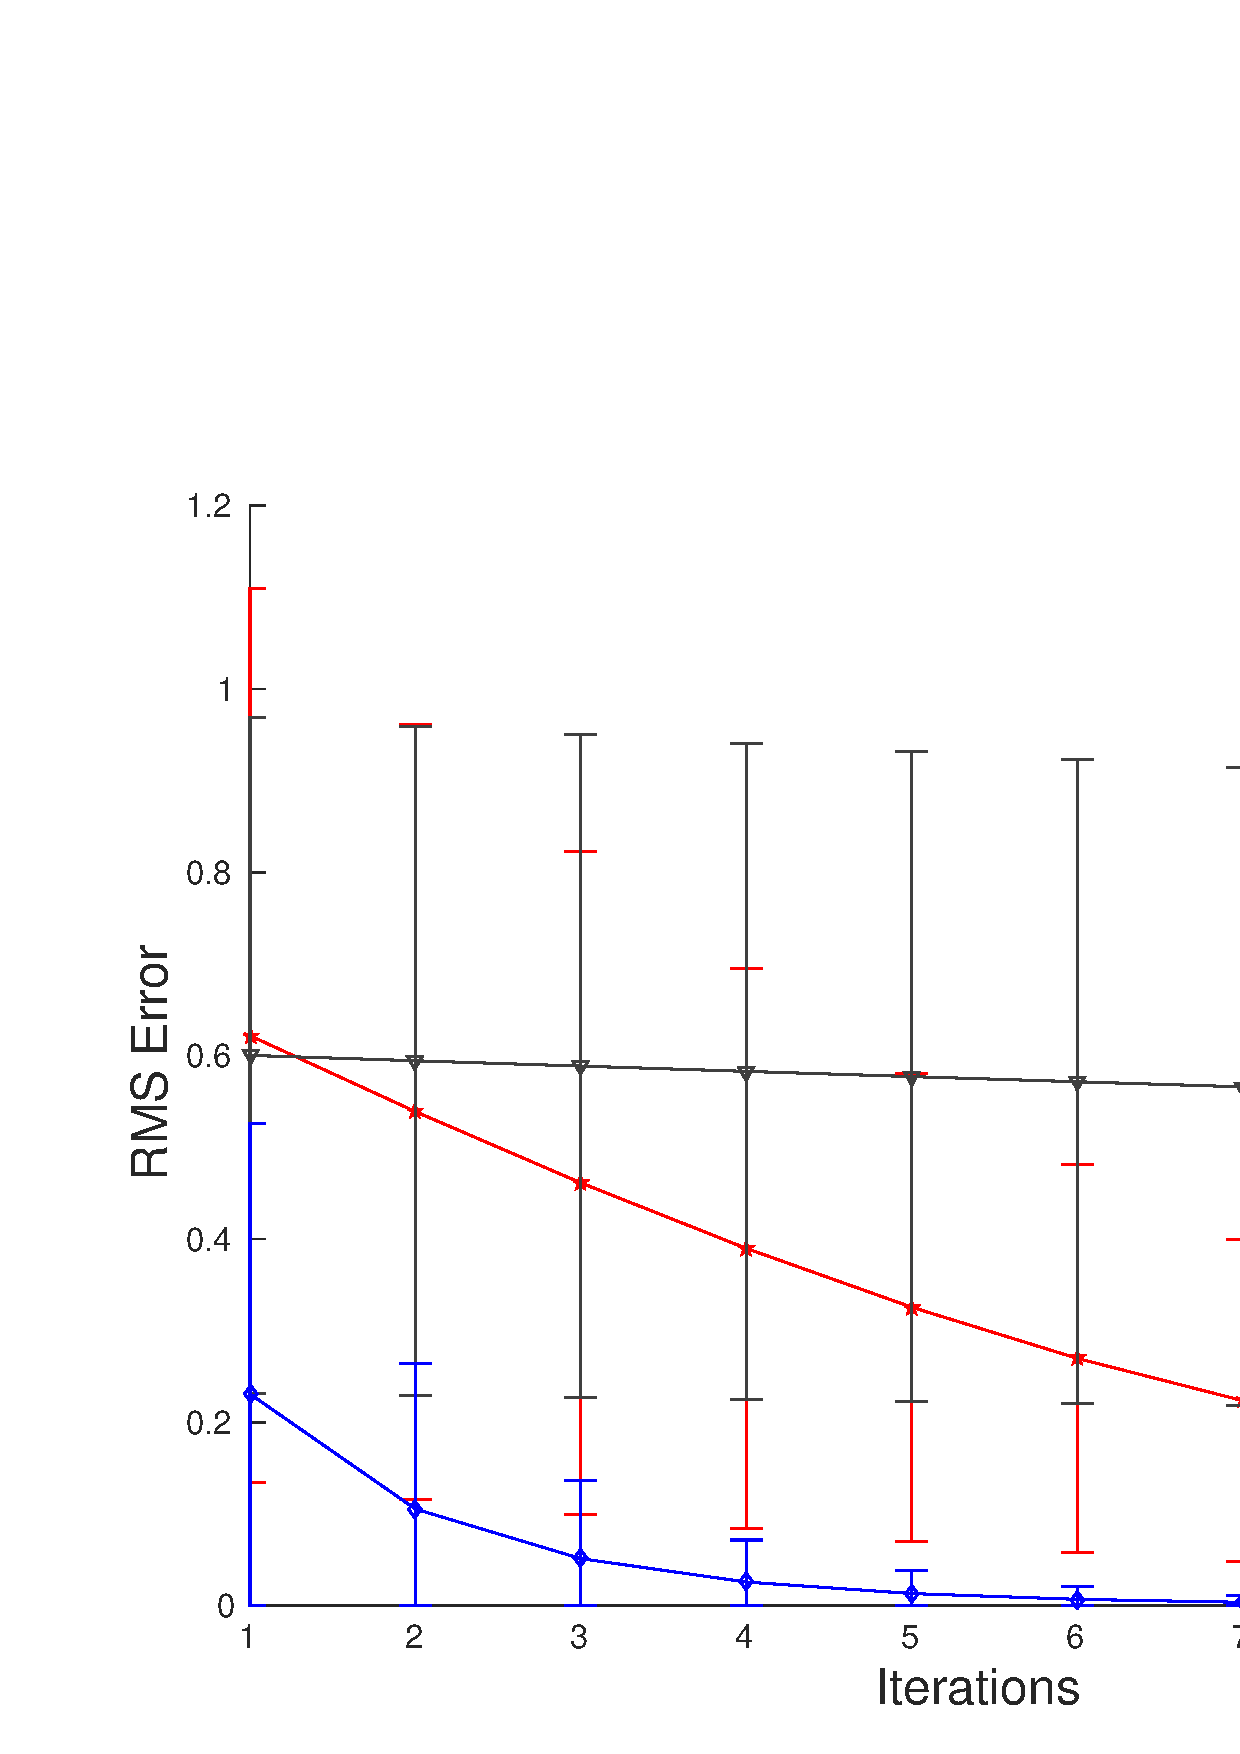
\includegraphics[width=0.3\linewidth]{putting1.pdf}
\label{fig:subfig2}}
\caption{The initial attempt falls short of the reference trajectory. We then modify the weights of the DMP to compensate for the modeling errors. The ball will then approach the hole, shown as a thick blue line at a distance of 0.5 meters, with approximately zero velocity.} 
\label{putting1} 
\end{figure}
\end{frame}
%
\begin{frame}{Toy Example: Putting}
\begin{figure}
\centering
%\includegraphics[scale=0.50]{comparison.eps}
\newlength\figureheight 
\newlength\figurewidth 
\setlength\figureheight{6cm}  
\setlength\figurewidth{6cm} 
\scalebox{0.8}{% This file was created by matlab2tikz.
% Minimal pgfplots version: 1.9
%
%The latest updates can be retrieved from
%  http://www.mathworks.com/matlabcentral/fileexchange/22022-matlab2tikz
%where you can also make suggestions and rate matlab2tikz.
%
\begin{tikzpicture}

\begin{axis}[%
width=0.95092\figurewidth,
height=\figureheight,
at={(0\figurewidth,0\figureheight)},
scale only axis,
separate axis lines,
every outer x axis line/.append style={black},
every x tick label/.append style={font=\color{black}},
xmin=0,
xmax=12,
xlabel={Iterations},
every outer y axis line/.append style={black},
every y tick label/.append style={font=\color{black}},
ymin=-0.05,
ymax=0.4,
ylabel={RMS Error},
title={Learning Performance in Putting},
legend style={legend cell align=left,align=left,fill=white}
]
\addplot [color=blue,solid]
 plot [error bars/.cd, y dir = both, y explicit]
 table[row sep=crcr, y error plus index=2, y error minus index=3]{%
1	0.233032343134884	0.118115271422138	0.118115271422138\\
2	0.0924719913705091	0.0562589335711811	0.0562589335711811\\
3	0.0384258808828579	0.0276274441478736	0.0276274441478736\\
4	0.0165387503761337	0.0138614543017086	0.0138614543017086\\
5	0.00733384353006482	0.00703352539176592	0.00703352539176592\\
6	0.00333781167932676	0.00358523371207059	0.00358523371207059\\
7	0.00155369907429323	0.0018294817119812	0.0018294817119812\\
8	0.000737146368162867	0.000933121803618784	0.000933121803618784\\
9	0.000355312489801426	0.000475460765776891	0.000475460765776891\\
10	0.000173512604061655	0.000241998267982427	0.000241998267982427\\
};
\addlegendentry{wILC};

\end{axis}
\end{tikzpicture}%}
\caption{Convergence is quadratic for the simulated scenario where we have unknown inertial disturbances acting on the motors.}
\label{wILCTrajectoryPutting}
\end{figure}
\end{frame}
%
\begin{frame}{Goal based ILC 1/2}
\begin{itemize}
\item Task performance depends only on reaching the desired position and velocity at the right time.
\end{itemize}
\begin{equation}
\begin{aligned}
\ValueFunction(\sysInput_L) &= \error_{N}^{\mathrm{T}}\vec{Q}_{N}\error_{N}, \\
&= (\vec{F}_N\sysInput_L + \linDist_N)^{\mathrm{T}}\vec{Q}_{N}(\vec{F}_N\sysInput_L + \linDist_N), \\
\vec{F}_N &= 
 \begin{bmatrix}
  \vec{A}_{N-1} \ldots \vec{A}_2 \vec{B}_1 & \cdots & \vec{B}_N 
 \end{bmatrix}.
\end{aligned}
\end{equation}
\begin{itemize}
\item $\vec{F}_{N}$ is the block row entry of $\vec{F}$ corresponding to the hitting time $t = N$
\end{itemize}
\begin{equation}
\begin{aligned}
\sysInput_{k+1} &= \sysInput_k - (\vec{F}^{\mathrm{T}}\vec{M}\vec{F})^{-1}\vec{F}^{\mathrm{T}}\vec{M}\error_k.
\end{aligned}
\end{equation}
\begin{itemize}
\item $\vec{M}$ has all the diagonal entries $\vec{Q}_{t}$ set to zero except for the last block entry $\vec{Q}_{N}$ corresponding to hitting time.
\end{itemize}
\end{frame}
%
\begin{frame}{Goal based ILC 2/2}
\begin{itemize}
\item Execution errors in tracking the rhythmic DMP prevents us from initializing the robot at each iteration to the same state.
\item To compensate for the varying initial conditions we recompute the reference control input $\sysInput_{\mathrm{IDM}}$ by starting the movement primitive from the current state.
\end{itemize}
\begin{equation}
\begin{aligned}
\sysInput_{\mathrm{TOT}} &= \sysInput_{\mathrm{FB}} + \sysInput_{\mathrm{FF}}, \\
\sysInput_{\mathrm{FF}} &= \sysInput_{\mathrm{IDM}} + \sysInput_{k+1}, \\
\sysInput_{k+1} &= \sysInput_k - \beta((\vec{F}^{\mathrm{T}}\vec{M}\vec{F})^{-1}\vec{F}^{\mathrm{T}}\vec{M} + \vec{K}_{\mathrm{LQR}})\error_{k}.
\end{aligned}
\end{equation}
\begin{itemize}
\item $\vec{M}$ can be designed to consider not just the hitting state, but
a hitting segment of the rhythmic DMP.
\item $\beta \in (0,1]$ is the learning rate.
\end{itemize}
\end{frame}
%
\begin{frame}{ILC lessons taken and tips for the practicioner}
\begin{itemize}
\item Robustly stabilizing feedback in the parallel loop. At the cost of larger initial error, we suggest increasing the input penalties on the LQR to ensure stability of ILC in robotics applications.
\item Reduced sampling rate increases the margins for monotonic stability. Considering only a hitting segment likewise in our application makes our approach stable.
\item Rhythmic DMPs can be useful for representing striking motions.
\item Current-iteration ILC can be added serially to predictive ILC.
\end{itemize}
\end{frame}
%
\end{document} 